\section{Demonstration des Programms}
\begin{frame}{\insertsection}
	\begin{figure}
		\animategraphics[autoplay,loop,width=\linewidth]{30}{images/GIFs/cantina/cantina-}{1}{827}
		\caption*{Applikation \it{Wavedit}, Github: \href{https://github.com/gooosz/Wavedit.git}{https://github.com/gooosz/Wavedit.git}}
	\end{figure}
\end{frame}

% Nochmal als Bilder falls Gif zu schnell für Erklärungen war
\begin{frame}{\insertsection}
	\begin{figure}
		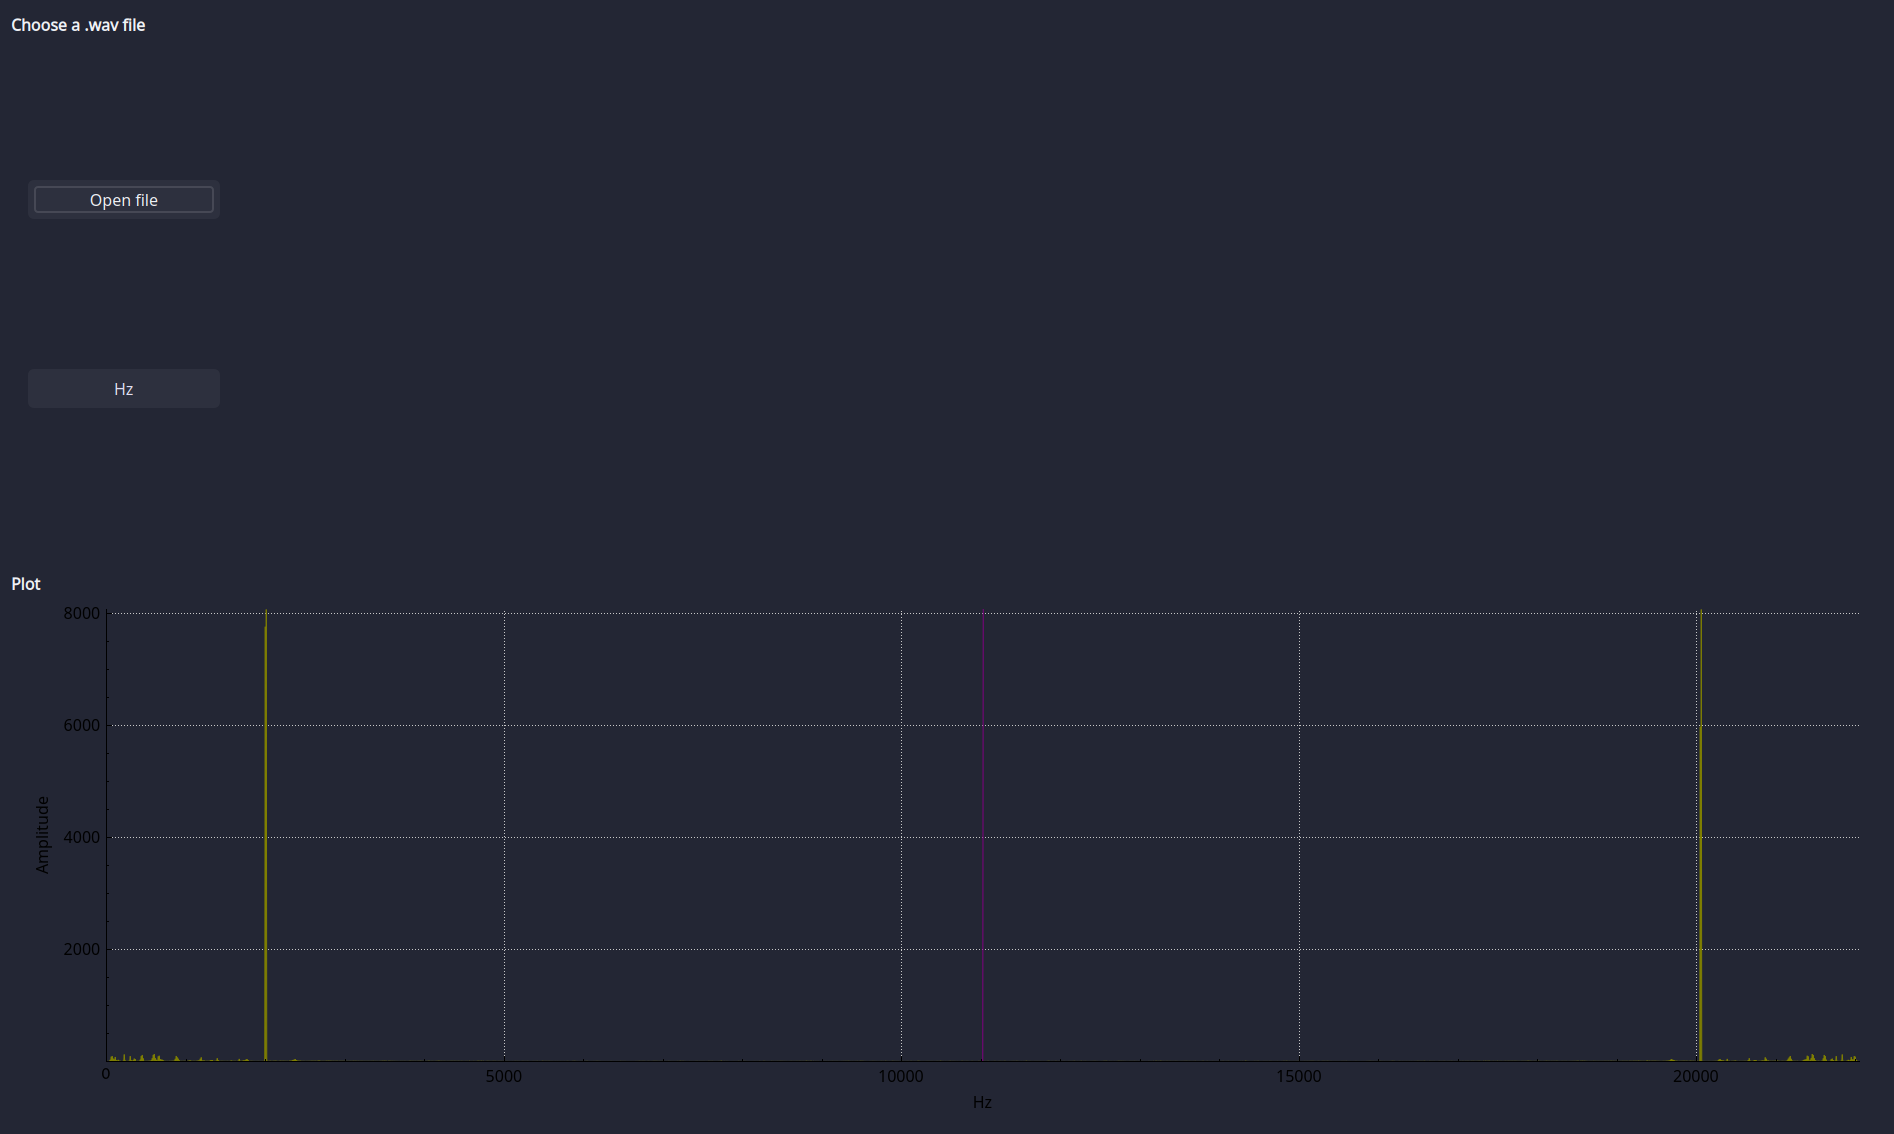
\includegraphics[width=\linewidth]{images/sin+cantina.png}
		\caption*{Frequenzspektrum von WAV Datei}
	\end{figure}
\end{frame}
\begin{frame}{\insertsection}
	\begin{figure}
		\includegraphics[width=\linewidth]{images/sin+cantina\_filtered.png}
		\caption*{Frequenzspektrum nach Filtern einer Frequenz von WAV Datei}
	\end{figure}
\end{frame}